\documentclass[12pt,reqno]{amsart}
\usepackage{./header, amssymb}

\hdr{Mathematical Statistics}{Chapter 12: Probabilistic graphical models}

\begin{document}

\bigskip

\prob Suppose that we have three binary random variables $X$, $W$, and $H$, which indicate whether a person exercises regularly ($X$), whether they are overweight ($W$), and whether they have heart disease ($H$). Discuss several causal structure involving these variables.

\bigskip
\textcolor{red}{We first might believe that $X$ is a confounding variable in the relationship between $W$ and $H$, meaning the causal graph has the form $W \leftarrow X \rightarrow H$. This means a person's decision to exercise has a direct influence on both their weight and whether they have heart disease, and that any statistical correlation between the latter variables is the result of this common cause and not a result of a direct cause and effect relationship between the two. Alternatively, we might believe that $X$ serves as a mediating variable between $W$ and $H$, meaning the causal graph has the form $W \to X \to H$. This means that a person's weight directly influences their decision to exercise, and then this latter decision directly influences whether they have heart disease. However, this causal model still assumes there is not a direct cause and effect relationship between $W$ and $H$.}
\bigskip













\prob Let $X$ and $Y$ be binary random variables that indicate whether a person has \textit{hydromechanical trepidation syndrome} ($X$) and whether they test positive ($Y$) for it. Suppose that
	\[p(y=1 |x=1) = 0.98 \quad \text{and} \quad p(y=1 | x=0) = 0.1.
	\]
Express the flow of information from $X$ to $Y$ as a stochastic link by explicitly writing down a link function.

\bigskip
\textcolor{red}{The link from $X$ to $Y$ is given by
	\[Y \mid X \sim \mathcal{B}er(\theta), \quad \theta = g(x) = 0.1(1-x) + 0.98x.
	\]}
\bigskip
	







\prob Explicitly draw the full graphical structure for a plated linear regression model

\bigskip
\begin{center}
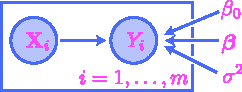
\includegraphics[scale=1.5]{lin-reg-00-plated.pdf}
\end{center}
\bigskip

when $m=3$.

\bigskip
\textcolor{red}{See your solutions from class.}
\bigskip

\end{document}